\documentclass{amsart}
\usepackage{amssymb}
\usepackage{hyperref,graphicx}
\usepackage{fmrtexcommon}

\DeclareMathOperator{\Inf}{Inf}
\DeclareMathOperator{\Act}{Act}
\DeclareMathOperator{\ap}{AP}
\DeclareMathOperator{\true}{\mathtt{true}}
\DeclareMathOperator{\false}{\mathtt{false}}

\DeclareMathOperator{\Pre}{Pre}
\DeclareMathOperator{\Post}{Post}

\theoremstyle{plain}
%%\newtheorem{thm}{Theorem}[section]
\newtheorem{thm}{Theorem}
\theoremstyle{definition}
\newtheorem{defn}{Definition}
\theoremstyle{definition}
\newtheorem{examp}{Example}


\begin{document}
\title{Introduction to Formal Methods for Robotics}
\author{Scott C. Livingston}
\thanks{\textit{Email}: \href{mailto:slivingston@cds.caltech.edu}{slivingston@cds.caltech.edu}}
\date{\textbf{draft}. \now{} (local time)}
\begin{abstract}
This paper provides a concise, self-contained introduction to 
topics usually regarded as ``formal methods for robotics.''  We assume the reader
has background knowledge broadly associated with robotics research, e.g., of
classical (linear) control theory, elementary graph search methods, and
propositional (Boolean) logic.
\end{abstract}
\maketitle

\section{Introduction}\label{sec:intro}

Historically, the phrase ``formal methods'' refers broadly to techniques for the
verification and synthesis of computer programs.  Research about hybrid systems
during the last twenty or so years came to include notions from formal methods
research, and unifying principles like that of bisimulation have been
recognized.  Somewhat more recently, these ideas have been introduced into
robotics.  Because much of the notation and core theory is apparently distinct
from comparably well-established areas of research in robotics, a concise
introduction for those working in other areas could be useful.  The present
paper seeks to provide this.  Fundamentally, the intent is to improve
accessibility, whether as a user, a reviewer, or a contributor.

%% While specific references will be given throughout, this does not aim to be a
%% survey.  There are several textbook treatments of the topics touched upon by
%% this introduction. These could be followed for more depth, more tutorial
%% derivations, etc.  Several books to consider are
%% \begin{itemize}
%% \item \cite{Hopcroft1979} --- finite languages and an early introduction to theoretical computer science.
%% \item \cite{Clarke1999,Baier2008} --- model checking, including probabilistic models, binary decision diagrams, partial order reductions, and a variety of temporal logic.
%% \item \cite{ChosetLHKBKT2005}; \cite{LaValle2006} (especially Chapters~6 and 10).
%% \item \cite{Tabuada2009} --- simulation-oriented (or ``symbolic'') view of hybrid systems.
%% \end{itemize}


\section{Preliminaries and basic notation}\label{sec:prelim}

$\mathbb{Z}$ is the set of integers, and $\mathbb{Z}_{\geq 0}$ is the set of
nonnegative integers.

\subsection{Sets, relations, and functions}
Let $X$ be a set.  The cardinality of $X$ is denoted by $\lvert X \rvert$, and the
collection of all subsets of $X$ is denoted by $2^X$.  $X$ is said to be
\textit{singleton} if $\lvert X \rvert = 1$.  A \textit{partition} $\mathcal{P}$
of $X$ is a subset of $2^X$ such that for any $A,B\in \mathcal{P}$, $A\cap B =
\emptyset$ or $A=B$, and $\bigcup_{A\in \mathcal{P}}A = X$.  Let $Y$ be a set
(not necessarily distinct from $X$).  A subset $R\subseteq X\times Y$ is
sometimes called a \textit{relation} (between elements of $X$ and $Y$), and we
write
\[
R^{-1} := \left\{ (y,x) \mid (x,y)\in R \right\} .
\]
As in the previous equation, we use ``$:=$'' to mean ``is defined by'' or, in
the style of pseudocode, ``is set to''.

A subset $R\subseteq X\times X$ is said to be an \textit{equivalence relation}
if it satisfies the following conditions.
\begin{enumerate}
\item (reflexivity) for each $x\in X$, $(x,x)\in R$;
\item (symmetry) $(x,y)\in R$ if and only if $(y,x) \in R$; and
\item (transitivity) if $(x,y)\in R$ and $(y,z)\in R$, then $(x,z)\in R$.
\end{enumerate}
Let $R$ be an equivalence relation on $X$. For $x\in X$,
\[
[x] := \left\{ y\in X \mid (x,y)\in R \right\} .
\]
The sets $[x]$ are called \textit{equivalence classes}.  It can be verified that
they partition $X$.

To extend functions to subsets of their domains rather than only particular
elements, we will occasionally abuse notation by writing, given $f:X\rightarrow
M$ is a function from $X$ into $M$,
\[
f(A) := \bigcup_{a\in A}f(a) ,
\]
where $A\subseteq X$.  A function may also be called a ``mapping''.


\subsection{Graphs}

A \textit{directed graph} (or \textit{digraph}) $G=(V,E)$ is a pair, where
$E\subseteq V\times V$, and $V$ and $E$ are called the sets of \textit{vertices}
and \textit{edges}, respectively.  Elements of $V$ are also referred to as
\textit{nodes}.  When no confusion will result, we also refer to directed graphs
as ``graphs''.  (Undirected graphs are not treated in this paper.)

Let $v\in V$.  The set of predecessors is
\[
\Pre(v) := \{ u\in V \mid (u,v) \in E \} ,
\]
and the set of successors is
\[
\Post(v) := \{ u\in V \mid (v,u) \in E \}.
\]
For brevity, we also denote these by $Ev=\Pre(v)$ and $vE=\Post(v)$,
respectively.  The \textit{in-degree} of $v$ is $\lvert \Pre(v) \rvert$, and the
\textit{out-degree} of $v$ is $\lvert \Post(v) \rvert$.  The \textit{degree} of
$v$ is the sum of the in-degree and out-degree of $v$.  A \textit{path} is an
ordered tuple of vertices $\langle v_{0} , v_{1} , \ldots , v_{n} \rangle$ such
that for $i\in \{0, 1,\ldots, n-1\}$, $(v_{i} , v_{i+1})\in E$.  A
\textit{cycle} is a path such that $v_{0}=v_{n}$.


\subsection{Defining syntax}

When introducing notations like linear temporal logic (LTL), we will need to
define the syntax and the semantics.  Syntax concerns how expressions are
constructed, whereas semantics concerns the meaning and interpretation of
expressions thus constructed.  In this paper we use an abbreviated style that
mostly follows Backus-Naur form \cite{Pattis}.  For the unfamiliar reader, we
remark that syntax definitions are context-free grammars (CFGs).  Thus,
syntactically correct formulae are just strings in the language of a grammar.


\section{Regular languages}\label{sec:reglang}

Let $\Sigma$ be a finite set, often referred to as the ``alphabet.''  Elements
of $\Sigma$ are sometimes referred to as ``symbols,'' ``letters,'' or
``characters.''  Carrying this metaphor forward (it is standard in the computer
science literature), the binary operation of concatenation is defined on
characters of $\Sigma$ to form strings, and the (Kleene) closure resulting from
this together with the empty string $\epsilon$ yields the monoid of all finite
strings $\Sigma^{*}$.\footnote{A \textit{monoid} is a structure that meets all
  group axioms except the existence of inverses. We abuse notation by writing
  $\Sigma^{*}$ for the monoid instead of $(\Sigma^{*}, \cdot )$, where $\cdot$
  is taken as the concatenation operator.  As is standard, juxtaposition is used
  instead of writing the operator out explicitly, i.e., we write $\alpha\beta$
  instead of $\alpha\cdot\beta$ for strings $\alpha$ and $\beta$.} (Sometimes a
string is called a ``word.'')

A \textit{language} is a subset of $\Sigma^{*}$.  In Section~\ref{sec:omegalang}
this is extended to infinite strings.

\begin{defn}\label{def:nfa}
A \textit{nondeterministic finite automaton} (NFA) $A$ is a tuple $( Q, q_I,
\Sigma, \delta, F )$ where $Q$ is a set of states, $q_I$ is the initial state,
$\Sigma$ is the alphabet over which $A$ accepts input, $F\subseteq Q$ is a set
of accepting states (or ``final states''), and $\delta: Q\times\Sigma
\rightarrow 2^Q$ is a transition function.  A string $\sigma=\sigma_0 \sigma_1
\cdots \sigma_{n-1} \in\Sigma^{*}$ is said to be \textit{accepted} by $A$ if
there exists a (finite) sequence of states $q_0 , q_1 , \ldots q_n$ such that
$q_0 = q_I$, for each $i\geq 0$, $q_{i+1}\in \delta(q_i , \sigma_{i})$, and $q_n
\in F$.  An NFA is said to be \textit{non-blocking} if for all $q\in Q$ and all
$a\in \Sigma$, $\lvert\delta(q,a)\rvert\geq 1$.  A \textit{deterministic finite
  automaton} (DFA) is an NFA where for each state $q\in Q$ and each character
$a\in \Sigma$, $\lvert\delta(q,a)\rvert\leq 1$.
\end{defn}
The \textit{language} of a finite automaton $A$ is the set of strings that it
accepts.  It is commonly denoted by $L(A)$.  NFAs and DFAs have the same
expressibility.  More precisely, any DFA is an NFA by definition, and
conversely,
\begin{thm}[Theorem~2.1 in \cite{Hopcroft1979}, page~22]
Let $A$ be a nondeterministic finite automaton.  There exists a deterministic
finite automaton $B$ such that $L(A)=L(B)$.
\end{thm}

Regular expressions provide a means to describe languages by formulae.  As for
finite automata, an alphabet $\Sigma$ must first be fixed.  To be concrete, let
$\Sigma=\{0,1\}$.  Then a regular expression is a formula $\psi$ that describes
how finite sequences (strings) of $0$ and $1$ may be formed, and the language of
$\psi$---i.e., the set of strings conforming to $f$---is denoted by $L(\psi)$.
For instance, if $\psi=011^{*}$, then $L(\psi)$ is the set of all strings
beginning with $0$ and followed by one or more $1$ symbols.

Syntactically, a \textit{regular expression} is a formula $\psi$ defined by the
following grammar productions
\begin{equation}\label{eq:regexgramm}
\psi ::= a \mid \psi+\psi \mid \psi\psi \mid \psi^{*}
\end{equation}
where $a$ is any symbol in $\Sigma$.  Note that parenthesis can be used to
change or make clear precedence when evaluating a regular expression.
Parenthesis is omitted from \eqref{eq:regexgramm} for succinctness.  The last
(highest precedence) production is for the operator $^*$, which is known as the
Kleene closure.  Informally it means that the operand occurs zero or more times.
Some authors also define $\psi^{+}$ to indicate ``$\psi$ at least once.''
However, it is easily derived from \eqref{eq:regexgramm} by $\psi\psi^{*}$.
%% XXX: Though I did not find Kleene's theorem itself in \cite{Hopcroft1979},
%% Theorems 2.3 (on page 30) and 2.4 (on page 33) together with results showing
%% the equivalence of NFA with \epsilon-transitions to DFAs provide it.
%%
%% Another place to search for a statement or a reference to the original paper
%% by Kleene is the book Algebraic Theory of Automata by Abraham Ginzburg (?).
\begin{thm}[Kleene's theorem]\label{thm:redfa}
For any regular expression (RE) $\psi$, there exists a deterministic finite
automaton (DFA) $A$ such that $L(\psi)=L(A)$.  Conversely, for any DFA $A$,
there exists a RE $\psi$ such that $L(\psi)=L(A)$.
\end{thm}

\begin{examp}
Let the alphabet be $\Sigma=\{\mathrm{a},\mathrm{b}\}$, and consider the regular
expression $\psi = (\mathrm{a}+\mathrm{b})^{*}\mathrm{a}$.  A deterministic
finite automaton $A$ that such that $L(A)=L(\psi)$ is shown in
Figure~\ref{fig:smalldfa}.
\begin{figure}
\centering
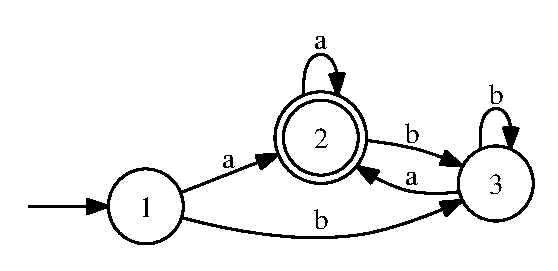
\includegraphics[width=7cm]{figures/exampleDFA.eps}
\caption{Deterministic finite automaton recognizing
  $(\mathrm{a}+\mathrm{b})^{*}\mathrm{a}$. The start state is indicated by an
  arrow without a base, and accepting states are double-bordered.  Using the
  notation from the text, the initial state is $q_I = 1$, and any string
  terminating at a state in $F=\{ 2 \}$ is accepted.}
\label{fig:smalldfa}
\end{figure}
\end{examp}

A classic introduction to the basic theory of automata that recognize languages
of finite strings is given by Hopcroft and Ullman \cite{Hopcroft1979}.  A
thorough algebraic treatment, including results about semiautomata and
equivalences to semigroups, has been given by Ginzburg \cite{Ginzburg1968}.
Holzer and Kutrib provide a recent survey \cite{HolzerK2011}.


\section{$\omega$-regular languages}\label{sec:omegalang}

In this section, languages of strings of infinite length are considered in a
manner that extends the treatment of Section~\ref{sec:reglang}.  Let $\Sigma$ be
a finite set.  Again, $\Sigma$ is commonly referred to as the ``alphabet.''
Denote by $\Sigma^{\omega}$ the set of all strings of countably infinite length,
or equivalently, all mappings of the nonnegative integers into $\Sigma$.  Let
$\sigma \in \Sigma^{\omega}$.  From the mapping, where $\sigma: \mathbb{Z}_{\geq
  0} \rightarrow \Sigma$, we obtain an infinite sequence (string) by writing the
parameter as a subscript, as in $\sigma_i = \sigma(i)$.  Subsets of
$\Sigma^{\omega}$ are termed \textit{languages}.

The finite automata in Section~\ref{sec:reglang} (cf.\ Definition~\ref{def:nfa})
are extended to operate on infinite-length strings by introducing new acceptance
conditions, which are listed below.  We begin with a definition in terms of a
particular such condition, and then list the others.  We assume without loss of
generality that automata are non-blocking, i.e., there is an infinite execution
for any string (though it is not necessarily accepted).
\begin{defn}
A \textit{nondeterministic B\"uchi automaton} (NBA) $\mathcal{A}$ is a tuple $( Q,
q_I, \Sigma, \delta, F )$, where the components are the same as in
Definition~\ref{def:nfa} except for the acceptance condition, which is
defined as follows.  A \textit{run} of $\mathcal{A}$ given a string
$\sigma\in\Sigma^{\omega}$ is an infinite sequence of states $\rho = \rho_0 \rho_1 \rho_2
\cdots$ such that $\rho_0 = q_I$ and for each $i\geq0$, $\rho_{i+1}\in \delta(\rho_i , \sigma_{i})$.  A string $\sigma\in\Sigma^{\omega}$ is said to be
\textit{accepted} by $\mathcal{A}$ if there is a run $\rho$ on $\sigma$ such
that $\Inf(\rho)\cap F\neq \emptyset$, where
\begin{equation}
\Inf(\rho) = \left\{ q\in Q \mid \forall i \exists j>i : \rho_j = q \right\} .
\end{equation}
\end{defn}
A \textit{deterministic} B\"uchi automaton is defined in the obvious way, i.e.,
where $\delta$ maps to singleton sets.  There are other possible acceptance
conditions, several of which we now list.  These are collectively known as
$\omega$-automata.  When an $\omega$-automaton has one of these acceptance
conditions, it is referred to by that condition, e.g., ``Rabin automaton.''
Let $\sigma\in \Sigma^{\omega}$, and let $\rho = \rho_0 \rho_1 \rho_2 \cdots \in
Q^{\omega}$ be a run of the automaton $\mathcal{A}$. Then, $\mathcal{A}$ accepts
$\sigma$ if\ldots
\begin{description}
\item[B\"uchi] $\Inf(\rho)\cap F \neq\emptyset$, where $F\subseteq Q$.

\item[co-B\"uchi] $\Inf(\rho)\cap F = \emptyset$, where $F\subseteq Q$.

\item[generalized B\"uchi] $\Inf(\rho)\cap F_i \neq\emptyset$ for all $F_i \in \mathcal{F}$ ($\mathcal{F}$ is finite).

\item[Muller] $\Inf(\rho)\in \mathcal{F}$, where $\mathcal{F}\subseteq 2^{Q}$.

\item[Rabin] there exists $(L_i , U_i)\in\mathcal{F}$ such that $\Inf(\rho)\cap L_i \neq \emptyset$ and $\Inf(\rho)\cap U_i = \emptyset$, where $\mathcal{F}\subseteq 2^{Q}\times 2^{Q}$.

\item[Streett] (the complement of Rabin acceptance) for all $(L_i , U_i)\in\mathcal{F}$, $\Inf(\rho)\cap L_i = \emptyset$ or $\Inf(\rho)\cap U_i \neq \emptyset$ (equivalently, $\Inf(\rho)\cap L_i \neq \emptyset$ implies $\Inf(\rho)\cap U_i \neq \emptyset$).

\item[parity] $\min \left\{ \chi(q) \mid q\in \Inf(\rho)\right\} $ is even, where $\chi:Q\rightarrow \mathbb{Z}$ assigns a color (integer) to each state of $\mathcal{A}$.
\end{description}

Unlike the finite automata discussed in Section~\ref{sec:reglang}, determinism
is not equivalent to nondeterminism for B\"uchi automata.  That is,
\begin{thm}
There exists a nondeterministic B\"uchi automaton $A$ such that $L(A)$ is not
the language of any deterministic B\"uchi automaton.
\end{thm}
On the other hand, nondeterministic B\"uchi automata (NBA) are equivalent to
automata of the other types of acceptance above, both deterministic and
nondeterministic.  For proofs, consult e.g., \cite{Gradel2002}.  There is an
algorithm known as Safra's construction for determinization of a NBA
\cite{Safra1988}.  Determinization is hard in the sense that, given a
nondeterministic B\"uchi automaton of size $n$, the deterministic Rabin
automaton resulting from Safra's construction has $2^{O(n\log n)}$ states
\cite{Safra1988}.  It is optimal in the sense that a lower bound the worst-case complexity 

%% Definition of omega-regular, and theorem that the above but not DBA recognize
%% exactly omega-regular languages.


\section{Temporal logic}\label{sec:tl}

The seminal paper introducing the use of temporal logic for program analysis is
\cite{Pnueli1977}.  We will focus on propositional linear temporal logic (LTL)
and fragments of it.  Nonetheless there are many other possibilities, including
variants of LTL that describe past events \cite{Emerson1990}. Also, LTL is not
the most expressive (e.g., \cite{Wolper1983}).  A few other prominent
specification languages are mentioned at the end of this section.  The
construction here is in terms of atomic propositions, which informally are
indivisible things that can be either $\true$ or $\false$.  This could
equivalently be done in terms of variables over finite domains, e.g., at each
time step, $y$ is assigned a value from $\{0,1,2\}$.  A significant alternative
is Lamport's ``Temporal Logic of Actions'' \cite{Lamport1994}.
\begin{examp}
Let $\ap = \{ p, q \}$.  Then $2^{\ap} = \left\{ \emptyset, \{p\}, \{q\} ,
\{p,q\}\right\}$.  The set $\{ p \}$ is regarded as the state of $p$ being
$\true$ and $q$ being $\false$.
\end{examp}
Let $\ap$ be a finite set of atomic propositions.  Syntax of LTL is obtained
from the grammar
\begin{equation}\label{eq:ltlgramm}
\varphi ::= \true \mid p \mid \varphi \vee \varphi \mid \neg \varphi \mid \Xnext \varphi \mid \varphi \Uuntil \varphi
\end{equation}
where $p\in\ap$.  Derived from these, we have
\begin{align*}
\false & := \neg \true \\
\varphi \wedge \varphi & := \neg \left( \neg \varphi \vee \neg \varphi \right ) \\
\varphi \implies \varphi & := \neg \varphi \vee \varphi \\
\Feventually \varphi & := \true \Uuntil \varphi \\
\Galways \varphi & := \neg \Feventually \neg \varphi ,
\end{align*}
any of which can be used as ``$\varphi$'' in the productions of
\eqref{eq:ltlgramm}.  Checking consistency of these syntactic derivations with
the semantics below is left to the reader.  Recall our introduction of infinite
strings in Section~\ref{sec:omegalang}.  Let $\Sigma=2^{\ap}$.  Now each
$\sigma\in \Sigma^{\omega}$ can be regarded as a mapping taking the nonnegative
integers into configurations of the atomic propositions.  The semantics of LTL
as built from the syntax above is defined recursively over productions from
\eqref{eq:ltlgramm}---together with several derived operators for clarity---as
follows.  The core operator for comparing strings with formulae is $\models$,
which is known as \textit{satisfies} (or \textit{models}).  Let $\sigma=\sigma_0
\sigma_1 \sigma_2 \cdots \in \Sigma^{\omega}$, and denote substrings by
\[
\sigma_{k:l} = \sigma_{k}\sigma_{k+1}\cdots\sigma_{l} ,
\]
where $k\leq l$ and $l$ may be omitted or $\infty$ to indicate the remainder of
$\sigma$ after the character at index $k$.  Define
\begin{enumerate}
\item $\sigma \models \true$ always (i.e., for $\sigma$);
\item $\sigma \models p$ iff $p\in \sigma_0$;
\item $\sigma \models \neg \varphi$ iff $\sigma\models\varphi$ is false, which is denoted by $\sigma \not\models \varphi$;
\item $\sigma \models \varphi \vee \psi$ iff $\sigma \models \varphi$ or $\sigma \models \psi$;
\item $\sigma \models \Xnext \varphi$ iff $\sigma_{1:} \models \varphi$;
\item $\sigma \models \varphi\Uuntil \psi$ iff either $\sigma\models\psi$ or there exists $j > 0$ such that for all $i$ where $0\leq i<j$, $\sigma_{i:}\models \varphi$ and $\sigma_{j:}\models \psi$;
\item $\sigma \models \Feventually \varphi$ iff there exists $i\geq0$ such that $\sigma_{i:}\models \varphi$;
\item $\sigma \models \Galways \varphi$ iff for all $i\geq0$, $\sigma_{i:}\models \varphi$.
\end{enumerate}
With the above construction, the \textit{language} of an LTL formula $\varphi$
is the set of all strings (i.e., sequences of configurations of the atomic
propositions $\ap$) that satisfy $f$.  It is denoted by $L(\varphi)$.

The syntax for regular expressions of Section~\ref{sec:reglang} can be extended
for $\omega$-regular expressions by introducing $\alpha^{\omega}$, which
indicates countably infinite repetition of the regular expression $\alpha$.
\begin{examp}
Let $\ap=\{ p, q\}$, and consider the LTL formula $\Galways\Feventually p$.  Intuitively,
$L(\Galways\Feventually p)$ is the set of all sequences where $p$ occurs infinitely often.
E.g., $\{p\}^{\omega}=\{p\}\{p\}\cdots$ is the sequence where $p$ is always
$\true$ and $q$ is always $\false$.  Clearly $\{p\}^{\omega}\in L(\Galways\Feventually p)$.
A precise characterization is
\[
L(\Galways\Feventually p) = \left\{ \sigma\in 2^{\ap} \mid \forall i \exists j : j > i \wedge \left( p\in\sigma_j \right) \right\} .
\]
\end{examp}


% \subsection{Conversions to $\omega$-automata}\label{sec:converttoaut}

% Using temporal logic formulae in practice usually involves first converting to
% an $\omega$-automaton that recognizes the same language.  This automaton is used
% for control synthesis in Section~\ref{sec:clsyssynth}.  It can also be used
% for model checking \cite{VardiW1986}.  Noteworthy algorithms with implementations are
% \begin{itemize}
% \item LTL2BA (\url{http://www.lsv.ens-cachan.fr/~gastin/ltl2ba/}) by Gastin and Oddoux for LTL conversion to generalized B\"uchi or nondeterministic B\"uchi automaton \cite{GastinO2001};
% \item LTL2DSTAR (\url{http://www.ltl2dstar.de/}) by Klein for LTL conversion to deterministic Streett and Rabin automata \cite{KleinB2006}.
% \end{itemize}


% \subsection{Noteworthy fragments and variants}

% Broadly speaking, it is hard to support design specifications that can be
% arbitrary LTL formulae because of the exponential complexity of conversion from
% the formula to an automaton \cite{VardiW1986}.  E.g., several times for
% conversion on a simple yet practically well-motivated formula are provided in
% Table~1 of \cite{GastinO2001}; also cf.\ Section~7 of that paper.  An important
% effort is thus to find useful fragments of LTL, which are sometimes tailored to
% specific problem settings.

% A classification of types of formulae is given in \cite{MannaP1990}.

% An incomplete list of fragments and variants follows.
% \begin{itemize}
% \item GR(1) \cite{KestenPP2005,BloemJPPS2012}
% %% \item scLTL
% \item Metric Temporal Logic (MTL) \cite{KaramanF2008}
% \item Bounded Linear Temporal Logic (BLTL) \cite{ZulianiPC2010} (...or (Finkbeiner and Sipma, 2001), which is reference [8] in \cite{ZulianiPC2010}, may be better).
% \end{itemize}


% \subsection{Besides LTL}

% Aside from linear-time, another prominent view of program execution is that of
% \textit{branching-time}.  Roughly speaking, a branching-time logic allows
% formulae to describe the existence of paths.  For instance, one can assert that
% a property will eventually hold under some execution beginning from the current
% time.  By contrast, a linear-time logic like LTL describes properties that hold
% over all executions.  To make this precise, we must first introduce Kripke
% structures, which are special cases of the transition systems introduced in
% Section~\ref{sec:ts}.
% \begin{defn}\label{def:krips}
% Let $\ap$ be a finite set of atomic propositions.  A \textit{Kripke structure}
% is a tuple $\mathcal{M} = (S,s_0 , \mathcal{R},L)$ where $S$ is a finite set of
% states, $\mathcal{R}\subseteq S\times S$ is a transition relation, and
% $L:S\rightarrow 2^{\ap}$ is a labeling of the states. A \textit{path} of
% $\mathcal{M}$ is a sequence of states $\rho_0 \rho_1 \cdots$ such that $\rho_0 =
% s_0$ and for each $i\geq 0$, $(\rho_i , \rho_{i+1})\in\mathcal{R}$. A finite
% path is a finite sequence of states conforming to $\mathcal{M}$ in the same way.
% \end{defn}
% (Note that the model of Definition~\ref{def:krips} can be extended to have
% actions \cite{Clarke1999}, thus becoming similar to the transition system of
% Definition~\ref{def:ts}.)

%%Computation tree logic (CTL) %% XXX
%% is a branching-time logic defined syntactically by the grammar
%% \[
%% \varphi ::= \true \mid 
%% \]


%% XXX
%% \section{$\mu$-calculus}
%% \cite{EmersonJS2001}


\section{Transition systems}\label{sec:ts}

One utility of the theory presented in previous sections is the formal
description of properties held by a system.  For instance, we can formally say
that a print server, given enough ink, must always eventually complete printing
jobs using an LTL formula like
\[
\Galways\left(\mathtt{ink}\rightarrow \bigwedge_{i}\Galways\left( r_i \rightarrow \Feventually g_i \right)\right) .
\]
In the context of motion planning, we can formally say that a robot must reach
and remain within the $\mathrm{Goal}$ region while avoiding the
$\mathrm{Unsafe}$ region using a formula like $\Galways \neg\mathrm{Unsafe} \wedge
\Feventually\Galways \mathrm{Goal}$.  In the present setting, the thing for which we wish to
achieve or verify such properties is modeled by a transition system, as in the
following
\begin{defn}\label{def:ts}
A \textit{transition system} is a tuple $\mathcal{T} = (S,\Act, S_{\mathrm{Init}},
\longrightarrow, L, \ap)$ where $\ap$ is a finite set of atomic propositions, $S$
is a set of states,\footnote{$S$ is not to be confused with the states in
  Definition~\ref{def:nfa}.} $\Act$ is a set of sets of actions indexed by $S$,
$L:S\rightarrow 2^{\ap}$ is a labeling, $S_{\mathrm{Init}}\subseteq S$ is the
set of initial states, and $\longrightarrow\subseteq S\times\Act(S)\times S$ is
a transition relation.  Every possible transition $(s,a,s')\in \longrightarrow$
is consistent with $\Act$ in that we require $a\in\Act(s)$. A transition
$(s,a,s')\in\longrightarrow$ is also denoted by $s \overset{a}{\longrightarrow} s'$.

An \textit{execution} of a transition system is a sequence of states
$\rho=\rho_0 \rho_1 \cdots$ such that $\rho_0 \in S_{\mathrm{Init}}$ and for
each $i\geq 0$, there is an action $a\in\Act(\rho_i)$ such that $\rho_i
\overset{a}{\longrightarrow}\rho_{i+1}$.  A finite execution is a finite
sequence of states with the same conformance requirements as (infinite)
executions.

A \textit{trace} of a transition system $\mathcal{T}$ is a sequence of labels (subsets of
$\ap$) $\sigma=\sigma_0 \sigma_1 \cdots$ for which there exists an execution
$\rho$ of $\mathcal{T}$ such that $L(\rho_{i})=\sigma_{i}$ for $i=0,1,2,\ldots$.  A finite
trace is defined similarly but for some finite execution.
\end{defn}
Note that $S$ is not necessarily finite, and the transition relation
$\longrightarrow$ is not necessarily deterministic.  When special restrictions
are assumed, then the appropriate qualifier is included in the name, e.g., a
``deterministic transition system.''  The generality of this definition permits
comparison of finite transition systems with those taking states in
$\mathbb{R}^n$, which we introduce in Section~\ref{sec:conttodiscr}.  Given a
transition system $\mathcal{T}$, a natural question is how to select actions so that all
executions thus arising satisfy a desired property.  That is the problem of
\textit{formal synthesis}, and we introduce it and basic solution methods in
Sections~\ref{sec:clsyssynth} and \ref{sec:reactsynth}.

\begin{examp}
\begin{figure}
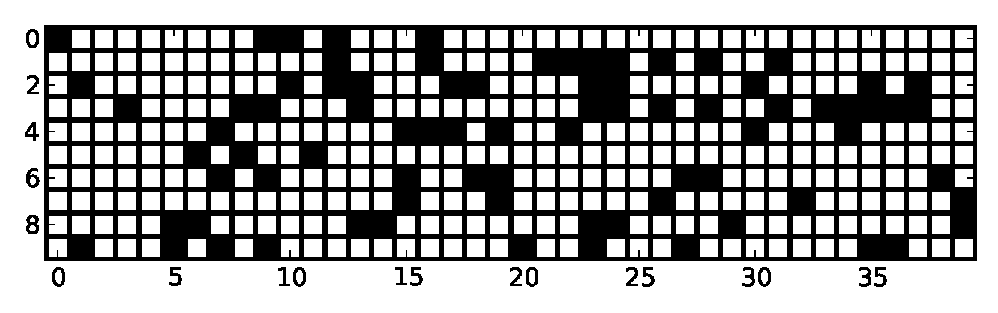
\includegraphics[width=9cm]{figures/illgridworld.eps}
\caption{Gridworld of size $10\times 40$.  Black blocks indicate impassable
  cells. Motion among unoccupied cells can be ``up,'' ``down,'' ``left,'' or
  ``right'' (known as 4-connected).  Diagonal motion may be available (known as
  8-connected).}
\label{fig:illgw}
\end{figure}
Gridworlds (sometimes referred to as ``block worlds'') are used for illustration
throughout the AI and robotics literature.  A small $10\times 40$ gridworld is
depicted in Figure~\ref{fig:illgw}.  At any (discrete) time, the robot is
assumed to occupy a single cell (a small white square in
Figure~\ref{fig:illgw}).  From there, it can move ``up,'' ``down,'' ``left,'' or
``right,'' except when this would lead into an obstacle (any black cell in
Figure~\ref{fig:illgw}).  Some authors also allow diagonal motion: ``up-left,''
``up-right,'' etc.  This gridworld can be modeled as a transition system
$\mathcal{T}=(S,\Act, S_{\mathrm{Init}}, \longrightarrow, L, \ap)$ as follows.
\begin{itemize}
\item $S$ is the set of grid cell positions, of the form $(i,j)\in S$ for $i=0,\ldots,9$ and $j=0,\ldots, 39$.
\item For each $s\in S$, $\Act(s) \subseteq \left\{ \mathtt{up}, \mathtt{down}, \mathtt{left}, \mathtt{right} \right\}$, where actions are not available depending on obstacles in neighboring cells.  Alternatively, we can restrict actions by the transition relation (below), and instead define a uniform action set $\Act = \left\{ \mathtt{up}, \mathtt{down}, \mathtt{left}, \mathtt{right} \right\}$, where we removed dependence on state.
\item $S_{\mathrm{init}}$ is the set of cells from which the robot may be begin execution.  E.g., this could be the bottom leftmost position, $S_{\mathrm{init}} = \{ (9,0) \}$.
\item For any states $s, s'$ and action $a$, $s \overset{a}{\longrightarrow} s'$ if and only if $s$ and $s'$ do not contain static obstacles, $s$ and $s'$ share a side, and $a$ is the physically appropriate action to cross that side.  E.g.,
\[
(9,0) \overset{\mathtt{up}}{\longrightarrow} (8,0)
\]
is a possible transition.
\item $\ap$ and $L$ depend on the task.  E.g., if the robot was supposed to visit the rightmost top and bottom cells infinitely often---as in a surveillance mission---then we could set $\ap=\{ \mathtt{goal}_1, \mathtt{goal}_2 \}$ and
\[
L(s) = \Bigg\{ \begin{array}{ll}
\{\mathtt{goal}_1 \} & \mathrm{if}\quad s = (0,39)\\
\{\mathtt{goal}_2 \} & \mathrm{if}\quad s = (9,39)\\
\emptyset & \mathrm{otherwise.} \\
\end{array}
\]
\end{itemize}
This can be extended to the 8-connected setting in the obvious way.  The state
could be modified to include orientation of the robot, in which case an action
for ``turning'' would be needed.
\end{examp}

If there is at most a single action available from every state (i.e., $\lvert
\Act(s) \rvert = 1$ for all $s\in S$), the question of control is irrelevant and
our focus becomes verification rather than control synthesis. When this is the
case, the action set $\Act$ will be omitted, and the transition relation
$\longrightarrow$ will be a treated as a subset of $S\times S$.


\section{Simulation}\label{sec:sim}

Given a complicated transition system, we may ask whether there is a transition
system that is simpler while preserving properties that we care about.  The
intuitive ``similarity'' here can be formalized by simulation relations as
follows.  We begin with the case where no actions (control inputs) are available.
\begin{defn}
Let $\ap$ be a set of atomic propositions, and let $\mathcal{T}_1=(S_1, S_{\mathrm{Init},1}, \longrightarrow_1, L_1 , \ap )$ and $\mathcal{T}_2=(S_2 , S_{\mathrm{Init},2}, \longrightarrow_2 , L_2 , \ap )$ be transition systems with trivial action sets.  A subset $R\subseteq S_{1}\times S_{2}$ is called a \textit{simulation relation} if
\begin{enumerate}
\item for all $(s_1, s_2)\in R$, $L_{1}(s_{1})=L_{2}(s_{2})$;
\item for each $s_{0,1} \in S_{\mathrm{Init},1}$, there exists $s_{0,2} \in S_{\mathrm{Init},2}$ such that $\left( s_{0,1}, s_{0,2} \right) \in R$;
\item for each $(s_1, s_2)\in R$, for all $s'_1 \in S_1$ where $s_{1}\longrightarrow s'_{1}$, there is some transition $s_{2}\longrightarrow s'_{2}$ in $\mathcal{T}_2$ such that $(s'_{1}, s'_{2})\in R$.
\end{enumerate}
When such a relation exists, we say that \textit{$\mathcal{T}_2$ simulates $\mathcal{T}_1$}, which is denoted by $\mathcal{T}_1 \preceq \mathcal{T}_2$.
\end{defn}
An immediate observation is that $\mathcal{T}_1 \preceq \mathcal{T}_2$ implies that every trace of
$\mathcal{T}_1$ is also a trace of $\mathcal{T}_2$.  (Recall traces from Definition~\ref{def:ts}.)
Thus a property that is verified for all traces of $\mathcal{T}_2$ must also hold for
$\mathcal{T}_1$.  Furthermore, a property that is satisfied by some trace of $\mathcal{T}_1$ is also
satisfied by some trace of $\mathcal{T}_2$.  Simulations are transitive, i.e., $\mathcal{T}_1
\preceq \mathcal{T}_2$ and $\mathcal{T}_2 \preceq \mathcal{T}_3$ implies $\mathcal{T}_1 \preceq \mathcal{T}_3$.

%% XXX: Should I mention Milner's book as the original?

The directionality of simulation should be obvious.  That is, one system
simulates another, but not necessarily the other way around.  When both
directions hold, it is called a bisimulation.  More precisely, given two
transition systems $\mathcal{T}_1$ and $\mathcal{T}_2$ and a relation $R\subseteq S_1 \times S_2$,
$R$ is called a \textit{bisimulation} if $R$ is a simulation relation from $\mathcal{T}_1$
to $\mathcal{T}_2$ and $R^{-1}$ is a simulation relation from $\mathcal{T}_2$ to $\mathcal{T}_1$.
Bisimulation is an equivalence relation on transition systems because any
transition system has the identity bisimulation relation with itself
(reflexivity), symmetry of bisimulation is obvious (merely swap the order of
$\mathcal{T}_1$ and $\mathcal{T}_2$ in the definition and then use the relation $R^{-1}$), and
transitivity is obtained from the transitivity of simulation.  Furthermore,
bisimulation between two transition systems $\mathcal{T}_1$ and $\mathcal{T}_2$ implies that the
traces of $\mathcal{T}_1$ are exactly those of $\mathcal{T}_2$.  An important problem is computing
the existence of simulations and bisimulations, and to that end, several
algorithms and computational complexity results are provided in
\cite{Baier2008},\cite{Tabuada2009}.
\begin{examp}
\begin{figure}
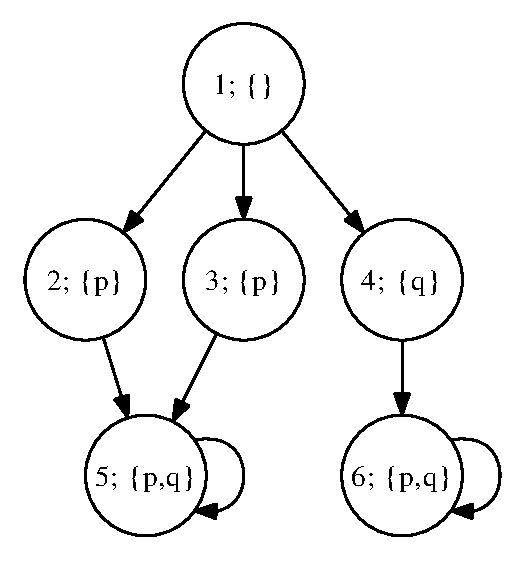
\includegraphics[width=5cm]{figures/exampleTS.eps}
\caption{A transition system where $S_{\mathrm{Init}}=\{ 1\}$, i.e., any execution must begin at node ``1''.  The set of atomic propositions is $\ap = \{ p,q\}$, and the labeling of each node is as indicated, e.g., $L(1) = \{\}$ (empty set, $\emptyset$).  The action set is trivial and thus not included.}
\label{fig:smallts}
\end{figure}

Consider the transition system $\mathcal{T}$ depicted in Figure~\ref{fig:smallts}.
$S_{\mathrm{Init}}=\{ 1\}$ and each state has labeling as indicated.  It should
be clear that only two traces are possible,
\begin{align*}
\emptyset \{p\} \{p,q\}^{\omega} \quad\mathrm{and}\quad \emptyset \{q\} \{p,q\}^{\omega} .
\end{align*}
In the first trace, execution begins at state~$1$ and both atomic propositions
are $\false$.  At the next time step, $p$ becomes $\true$, and after that, for
all remaining steps, both $p$ and $q$ are $\true$.  The second trace is similar
except that $q$ is $\true$ at the second time step, instead of $p$.

Intuitively we may expect that states $2$ and $3$ can be
aggregated somehow.  This is indeed possible using a bisimulation.  First,
consider the partition $\mathcal{P}$ of $S$
\[
\mathcal{P} = \left\{ \{1\}, \{2, 3\}, \{4\}, \{5\}, \{6\} \right\}.
\]
$\mathcal{P}$ defines an equivalence relation $\sim$ on $S$.  The only
non-singleton equivalence class is $[2] = [3] = \{2, 3\}$.  Let us decide
whether $\sim$ yields a bisimulation, where the other transition system is
$\mathcal{T}_{/\sim} = (\mathcal{P}, \{\{1\}\}, \longrightarrow_{/\sim}, L_{/\sim}, \ap)$.
Transitions in $\mathcal{T}_{/\sim}$ are defined by $[s]\longrightarrow_{/\sim} [s']$ if
and only if $s\longrightarrow s'$, and the labeling is $L_{/\sim}([s]) = L(s)$.
That the components of $\mathcal{T}_{/\sim}$ are well-defined is straightforward to verify.
The candidate relation $R$ is defined by $(s,[s])\in R$ for $s\in S$.  Again, we
see the only non-identity pairs are $(2,[2])$ and $(3,[2])$ (recall that
$[2]=[3]$).  Finally, the requirements for a bisimulation can each be verified
manually.  We sketch some of this process.
\begin{enumerate}
\item $L(2)=L(3)=\{p\}=L_{/\sim}([2])$.
\item The initial conditions are clearly satisfied because each transition system has only one initial state, and by definition of the relation, $(1, [1])\in R$ (recall that $[1]=\{1\}$ in this example).
\item Consider $(2,[2])$.  From state~$2$ there is a single transition to $5$. By construction, $[2]\longrightarrow_{/\sim}[5]$ is a transition in $\mathcal{T}_{/\sim}$, and $(5,[5])\in R$ as desired.  The same observation can be made for $(3,[2])$, where it is important to notice that $[3]\longrightarrow_{/\sim}[5]$ is the same transition as $[2]\longrightarrow_{/\sim}[5]$, by the definition of the equivalence class notation $[\cdot]$ (cf.\ Section~\ref{sec:prelim}).
\end{enumerate}
It follows that $R$ provides a bisimulation.  Practically we can instead study
the smaller transition system $\mathcal{T}_{/\sim}$, which is known as the \textit{bisimulation quotient}.
%% XXX: Is there an algorithm for computing this provided in (Baier and Katoen, 2008) or elsewhere that I should cite?
\end{examp}


\section{Closed systems synthesis}\label{sec:clsyssynth}

Let $\ap$ be a set of atomic propositions.  Given a transition system $\mathcal{T}$ and an
LTL formula $\varphi$ (known as the specification), both of which are in terms
of $\ap$, does there exist a policy for selecting actions such that all
executions of $\mathcal{T}$ satisfy $\varphi$?  More precisely, a \textit{control policy}
for $\mathcal{T}$ is a partial function $\pi:S^{*}S\rightarrow \Act(S)$ such that
\begin{enumerate}
\item $\pi$ is defined for all initial states $S_{\mathrm{Init}}$,
\item for any finite execution $\rho=\rho_0 \rho_1 \cdots \rho_i$ arising from $\pi$, $\pi(\rho)\in \Act(\rho_{i})$, i.e., $\pi$ selects a permissible action.
\end{enumerate}
An execution $\rho$ is said to \textit{conform} to $\pi$ if for all $i\geq 0$,
$\rho_{i}\overset{\pi(\rho_0 \rho_1 \cdots \rho_{i})}{\longrightarrow}
\rho_{i+1}$.  A trace $\sigma$ is said to \textit{conform} to $\pi$ if there is
an execution $\rho$ that yields $\sigma$ and $\rho$ conforms to $\pi$.  Thus,
the synthesis problem is to find a control policy $\pi$ such that all traces of
$\mathcal{T}$ conforming to $\pi$ satisfy (are in the language of) $\varphi$.  Note that
this problem is entirely analogous to that of Markov decision problems, except
that nondeterminism replaces stochasticity.

As mentioned in Section~\ref{sec:converttoaut}, the LTL formula $\varphi$ can be
converted to a deterministic $\omega$-automaton $\mathcal{A}_{\varphi}$ that
accepts precisely those strings satisfying $\varphi$.  Recall this is formally
stated as $L(\varphi)=L(\mathcal{A}_{\varphi})$.  Notice that the input of
$\mathcal{A}_{\varphi}$ is a string from $\Sigma^{\omega}$, which is exactly the
form of a trace of $\mathcal{T}$.  Intuitively then, we may expect to be able to treat
labels of states reached in an execution of $\mathcal{T}$ as being incrementally read by
$\mathcal{A}_{\varphi}$.  Thus, if we can find a manner for selecting actions so
that every trace is in the language of the automaton, then a solution to the
synthesis problem is obtained.  This approach is made precise with a product
automaton.  Here we only consider deterministic transition systems, i.e., those
for which there is exactly one succesor state for every action available from a state.
\begin{defn}
Let $\ap$ be a set of atomic propositions, let $\mathcal{T}=(S,\Act, S_{\mathrm{Init}}, \longrightarrow, L, \ap)$ be a deterministic transition system, and let $\mathcal{A}=( Q, q_I, 2^{\ap}, \delta, F )$ be a deterministic $\omega$-automaton.  (The acceptance condition need not be fixed here.)  The \textit{product automaton} $\mathcal{T}\times \mathcal{A}$ is a tuple $\left(Q', Q'_{\mathrm{Init}}, \delta' , F' \right)$ where
\begin{itemize}
\item $Q' := S\times Q$,
\item $Q'_{\mathrm{Init}} := S_{\mathrm{Init}}\times \{ q_I \}$,
\item $F' := S\times F$,
\item $\delta' \subseteq Q' \times Q'$, and $\left( (s,q), (s',q') \right)$ is in $\delta'$ if and only if $\delta(q, L(s)) = \{ q' \}$, and there is some action $a\in\Act(s)$ such that $s\overset{a}{\longrightarrow}s'$ is a transition in $\mathcal{T}$.
\end{itemize}
A run $\rho=(s_0 , q_0 ) (s_1 , q_1 ) \cdots$ of $T\times \mathcal{A}$ is accepted if $q_0 q_1 \cdots$ is accepted by $\mathcal{A}$.
\end{defn}
Notice that the product automaton has a trivial alphabet, which is omitted
entirely from the notation.  To obtain a control policy that ensures
satisfaction of the specification, it suffices to find an accepting run because
the states of $\mathcal{T}$ appearing in this run determine a finite-memory control
policy.  One way to obtain such a run in practice is to
\begin{enumerate}
\item regard actions of the deterministic transition system $\mathcal{T}$ as nondeterministic edges,
\item express it in the format appropriate for a model checker, such as Spin\footnote{\url{http://spinroot.com/spin/}} or NuSMV\footnote{\url{http://nusmv.fbk.eu/}},
\item assert the LTL formula $\neg \varphi$ and check whether it holds for all executions.
\end{enumerate}
Then, the model checker will either verify this claim, in which case there is no
control policy realizing the specification, or it will give a counter-example,
which can be translated into a control policy, as desired.


\section{Reactive synthesis}\label{sec:reactsynth}

Let $\mathcal{X}$ be a finite collection of ``input'' variables, and let
$\mathcal{Y}$ be a finite collection of ``output'' variables.  We assume these
sets are disjoint, i.e., $\mathcal{X}\cap \mathcal{Y} = \emptyset$.
%% Each
%% \textit{variable} $v$ has an associated \textit{domain} $\Sigma_{v}$ in which it
%% may take values.  A \textit{state} is an assignment of values to
%% variables. (Note there are multiple distinct uses of the word ``state.'')  It
%% should be clear that a state may also be regarded as an element of $\Sigma$.
Given an LTL formula $\varphi$ written in terms of $\mathcal{X}\cup
\mathcal{Y}$, construct a machine such that the input sequence, which the
machine does not control, and the output sequence together are in $L(\varphi)$.
This is called the problem of reactive synthesis. To the best of our knowledge,
it was first articulated by Church \cite{Church1962}, though without notions of
temporal and modal logic.
%% The problem is introduced in the manner as we have here and an
%% algorithm of double exponential complexity in the length of $\varphi$ is given
%% in \cite{PnueliR1989}.
We also refer to $\varphi$ above as the
``specification.''  In addition to being computationally hard, it is possible to
write noncausal specifications.  E.g., $(\Feventually x) \implies y$ is not practical
because in order to correctly set $y$ at the first time step, whether $x$ is $\true$
at a future time must be known.  Following the terminology of
\cite{PnueliR1989}, the (possibly adversarial) thing that selects values for
variables in $\mathcal{X}$ is termed the ``environment'' and the machine to be
designed is the ``system.''  Accordingly, we say that $\mathcal{X}$ are
environment variables, and $\mathcal{Y}$ are system variables.

\subsection{Time semantics}

A crucial aspect of reactivity is the relative timing of the system and the
environment.  We must decide when they can move and when a valuation (assignment
of values to variables) is declared as a state.  Let $\mathcal{X}$ and
$\mathcal{Y}$ be sets of environment and system variables, as introduced in the
previous section.  We consider two types of timing, which are based on two
transducer models that are defined below.  A Mealy time semantics allows the
$\mathcal{Y}$ variables to be assigned with knowledge of the current state and
the values that will be taken by the $\mathcal{X}$ variables at the next time
step.  Informally, the environment (which controls $\mathcal{X}$) selects its
next values using only the current state, and then the system (which controls
$\mathcal{Y}$) selects its next values both the current state and the
anticipated move by the environment.  By contrast, a Moore time semantics
requires all variables to be assigned values simultaneously, i.e., only as a
function of the current state.  The names ``Mealy'' and ``Moore'' follow the
names given to the following models, which provide the same time semantics in
the context of a finite-state machine that maps an input sequence to an output
sequence.  These are called \textit{transducers}.
\begin{defn}
A \textit{Mealy machine} is a tuple $\mathcal{M}:=\left(Q,q_{0},\Sigma_{I},\Sigma_{O},\delta,g\right)$,
with finite state set $Q$, initial state $q_0 \in Q$, and
where $\Sigma_{I}$ is a (finite) \textit{input alphabet}, $\Sigma_{O}$
is a (finite) \textit{output alphabet}, $\delta:Q\times\Sigma_{I}\rightarrow Q$
is a \textit{transition function}, and $g:Q\times\Sigma_{I}\rightarrow\Sigma_{O}$
is a \textit{output function}. Note that we abuse function notation
since $\delta$ and $g$ need not be defined for all state-input pairs,
i.e., elements of $Q\times\Sigma_{I}$.

A \textit{run} of a Mealy machine is a sequence of input-output pairs (or
equivalently, input-state pairs) that are consistent with transitions under
$\delta$. Input words, output words, and the machine language
$L\left(\mathcal{M}\right)$ follows from this.

Let $\mathcal{M}$ be a Mealy machine. $\mathcal{M}$ is said to be
\textit{input enabled} if \[
\forall q\in Q.\forall a\in\Sigma_{I}\left[\left(\exists b\in\Sigma_{O}.g\left(q,a\right)=b\right)\wedge\left(\exists q'\in Q.\delta\left(q,a\right)=q'\right)\right].\]
 $\mathcal{M}$ is said to be \textit{deterministic} if for all state-input
pairs, there is at most one output and at most one next state. (Note
that if $\mathcal{M}$ is both deterministic and input enabled, then
it maps every input word to a unique run.)
\end{defn}

\begin{defn}
A \textit{Moore machine} is tuple $\mathcal{M}:=\left(Q,q_{0},\Sigma_{I},\Sigma_{O},\delta,g\right)$,
where $Q$, $q_{0}$, $\Sigma_{I}$, $\Sigma_{O}$, and $\delta$
are defined as for Mealy machines, and where the output depends only
on state, i.e., $g:Q\rightarrow\Sigma_{O}$.
\end{defn}


\subsection{GR(1)}

Because of the difficulty of the general problem, there have been synthesis
problems posed in fragments of LTL.  We consider here Generalized Reactivity of
rank 1, commonly known as GR(1) \cite{KestenPP2005,BloemJPPS2012}.  It is
attractive because it has polynomial complexity in the number of states.  In
this context, a ``state'' is an assignment of the variables to particular
values.  However the number of states is exponential in the number of variables
(known as the curse of dimensionality), as will be shown by examples in
Section~\ref{sec:conttodiscr}.  Another fragment that is more expressive than
GR(1) and yet has similarly favorable complexity is Generalized Rabin(1)
\cite{Ehlers2011}.

Let $\mathcal{X}$ and $\mathcal{Y}$ be sets of Boolean variables.  For example,
at each time step $x\in\mathcal{X}$ has the value $\true$ or
$\false$.\footnote{This could be presented in terms of a set of atomic
  propositions and using subsets to indicate which are $\true$.  However, the
  present formulation in terms of variables is more common.}  The canonical
GR(1) formula is
\begin{equation}\label{eq:gr1}
  \theta^{\mathrm{env}} \wedge \Galways \rho^{\mathrm{env}} \wedge \left( \bigwedge_{j=1}^{m} \Galways\Feventually \varphi^{\mathrm{env}}_{j} \right) \implies \theta^{\mathrm{sys}} \wedge \Galways \rho^{\mathrm{sys}} \wedge \left( \bigwedge_{i=1}^{n} \Galways\Feventually \varphi^{\mathrm{sys}}_{i} \right)
\end{equation}
where
\begin{itemize}
\item $\theta^{\mathrm{env}}$ and $\theta^{\mathrm{sys}}$ are initial conditions;
\item $\rho^{\mathrm{env}}$ is a transition rule given as an LTL formula in terms of $\mathcal{X}\cup\mathcal{Y}\cup\Xnext\mathcal{X}$, where no other temporal operators appear;
\item $\rho^{\mathrm{sys}}$ is a transition rule in terms of $\mathcal{X}\cup\mathcal{Y}\cup\Xnext\mathcal{X}\cup\Xnext\mathcal{Y}$; and
\item $\varphi^{\mathrm{env}}_{j}$ and $\varphi^{\mathrm{sys}}_{i}$ are state formulae (i.e., lack temporal operators) in terms of $\mathcal{X}\cup\mathcal{Y}$.
\end{itemize}
The left side of \eqref{eq:gr1} is informally referred to as the assumption, and
the right side is the guarantee.  This terminology is motivated by a 2-player
game view of reactive synthesis in which we seek to build a discrete controller
that sets variables in $\mathcal{Y}$ so that the combined state sequence of
$\mathcal{X}$ and $\mathcal{Y}$ satisfies a desired property, given assumptions
about how the adversary (environment) may move.


%% XXX
% \section{2-player games on graphs}\label{sec:2pggames}

% Many of the control synthesis problems for finite transition systems that we
% have presented thus far can be reduced to parity games, which are a particular
% kind of 2-player game graph.  Intuitively, a game consists of two adversaries,
% referred to here as Player~0 and Player~1, and a graph with two types of
% vertices, $V_0$ and $V_1$, each corresponding to the respective player.  A play
% begins with a token being placed on an initial vertex and proceeds in turns,
% where Player~0 can select the next vertex if the token is on a vertex from
% $V_0$, and similarly for Player~1 if it is from $V_1$.  A play can be infinite
% or finite.  The latter occurs when the player who is to select the next vertex
% has no options.

%% XXX: mention memoryless determinacy (due to Zielonka?)


%% XXX
% \section{Probabilistic models}

% We develop the cases of probabilistic computation tree logic (PCTL) and
% probabilistic LTL describing control of Markov decision processes (MDPs).
% E.g., an introduction to Markov chains and MDPs sufficient for treating model
% checking is given in \cite{Baier2008}.  To fix notation, a discrete-time,
% finite state, labeled \textit{Markov decision process} $\mathcal{M}$ is a
% tuple $\left(S, \Act, L, \mathcal{P}\right)$ where $S$ is a finite set,
% $\Act$ is a set of actions (which may depend on state), $L:S\rightarrow
% 2^{\ap}$ is a labeling, and for each action $a$ defined at a state $s$,
% $\mathcal{P}_{s}^a$ is a next-state probability distribution over $S$.


\section{From uncountable to countable}\label{sec:conttodiscr}

Most treatments of the above topics in the computer science literature concern
sets that are at most countable.  However, dynamical systems are commonly framed
in Euclidean or similar spaces.  Exploring the mixing and interaction of these
two categories is the purview of hybrid systems research.  We only look here at
two approaches for treating continuous dynamical systems as discrete objects.
One nice entry point to alternative paths in hybrid systems---aside from
\cite{Tabuada2009} and the other textbooks mentioned in
Section~\ref{sec:intro}---is the Ph.D.\ thesis of M.S.~Branicky \cite{Branicky1995b}.

\subsection{Discrete abstractions}

The basic idea of a discrete abstraction is to partition the state space of a
dynamical system so that transitions among the parts are equivalent, in a sense,
to transitions among specific states within those parts.  In robotics, a similar
end is achieved using cell decompositions \cite{LaValle2006} (in particular,
Section~6.3, page~264).  However, cell decompositions are usually in terms of
the workspace, e.g., robot position but not velocity, whereas discrete
abstractions concern the entire state of hybrid systems \cite{AlurHLP2000}.  By
ensuring a bisimulation (cf.\ Section~\ref{sec:sim}) holds between the original
system and a discrete abstraction of it, verification or control synthesis for
one is the same as for the other, modulo some translation procedure.  A major
motivation for constructing the discrete absraction is that it may be viewed as
a finite graph, e.g., thus allowing reachability questions to be solved using
graph search algorithms.  While we do not explore it here, note that the notions
and techniques of abstraction are not necessarily discrete (e.g.,
\cite{PappasLS2000}).

We only consider here discrete-time, linear dynamical systems for simplicity of
presentation.  More sophisticated systems, including nonholonomic
\cite{Conner2006}, appear in the literature.  Begin with a trivial one-dimensional
\begin{examp}\label{eg:onedimds}
\begin{figure}
\setlength{\unitlength}{1.2cm}
\begin{picture}(6,1.7)(-1.5,-1)
\put(-1.5,0){\vector(1,0){5.5}}
\put(4.2,-.25){$\mathbb{R}$}
\put(0,-.25){\line(0,1){.5}}
\put(-1.3,-.75){$-1$}
\put(-1,-.25){\line(0,1){.5}}
\put(-.1,-.75){$0$}
\put(1,-.25){\line(0,1){.5}}
\put(.9,-.75){$1$}
\put(2,-.25){\line(0,1){.5}}
\put(1.9,-.75){$2$}
\put(3,-.25){\line(0,1){.5}}
\put(2.9,-.75){$3$}
\put(-.6,.17){$q_{-1}$}
\put(.4,.17){$q_{0}$}
\put(1.4,.17){$q_{1}$}
\put(2.4,.17){$q_{2}$}
%% \put(-.5,1.5){\circle{.5}}
%% \put(.5,1.5){\circle{.5}}
%% \thicklines
%% \put(-.25,1.5){\vector(1,0){.5}}
\end{picture}
\caption{State space for Example~\ref{eg:onedimds}.  The original dynamical
  system \eqref{eq:egonedimds} has trajectories in the interval $[-1,3[$ of the
  real line $\mathbb{R}$.  The discrete abstraction has four states, indicated
  by $q_{-1}$, $q_0$, etc.\ in the figure, corresponding to the intervals
  $[-1,0[$, $[0,1[$, etc.}
\label{fig:discab1dim}
\end{figure}

Consider a discrete-time, one-dimensional, linear dynamical control system that
has trajectories $x$ defined by the difference equation
\begin{equation}\label{eq:egonedimds}
x(t+1) = x(t) + u(t) ,
\end{equation}
where at each time step $t$, the state $x(t)$ is defined (constrained) to the
interval $\left[-1,3\right[$, i.e., $-1\leq x(t) < 3$, and the control input $\lvert u(t)
    \rvert \leq 1$.  Each trajectory must begin in the interval $[0,1[$.

A discrete abstraction based on unit intervals may be constructed as follows.
Define the transition system
\[
\mathcal{T}=\left( \{ q_{-1},q_{0},q_{1},q_{2} \}, \{ \mathtt{left}, \mathtt{stay}, \mathtt{right}\}, \{ q_0 \} , \longrightarrow , L, \ap \right) ,
\]
where $\ap = \{-1, 0, 1, 2\}$, $L:q_{i}\mapsto \{i\}$, and the actions $\Act$
and the transition relation $\longrightarrow$ are defined in the obvious way
according to the illustration in Figure~\ref{fig:discab1dim}.  $\mathtt{left}$
and $\mathtt{stay}$ are identified at $q_{-1}$, and similarly for
$\mathtt{right}$ and $\mathtt{stay}$ at $q_{2}$.  An example transition is
$q_{0}\overset{\mathtt{right}}{\longrightarrow} q_{1}$.

The state space of the original system, which is the uncountably infinite
interval $[-1,3[$, is related to the states of $\mathcal{T}$ using the floor function, by
\[
q_i \sim a \quad\textrm{if and only if}\quad i = \lfloor a \rfloor ,
\]
where $q_i$ is a state of $\mathcal{T}$ and $a$ is a state of the original
dynamical system (so, $-1\leq a < 3$).  If we regard the original dynamical
system as a transition system with intervals $[-1,0[$, $[0,1[$, etc.\ labeled
using $\ap$, then $\sim$ is a bisimulation relation.  Transitions in the 
original system (i.e., elements of the transition relation) are
state-input-next-state triples that trajectories are comprised of.  More
precisely, for any $a,b\in [-1,3[$ and $r\in [-1,1]$,
$a\overset{r}{\longrightarrow} b$ is a possible transition if and only if $b = a+r$.
As stipulated above, continuous state trajectories must begin in the leftmost
interval, i.e., $-1 \leq x(t) < 0$.  Thus an execution (as in
Definition~\ref{def:ts}) of the original system is a sequence of real numbers
\[
x(0)\overset{u(0)}{\longrightarrow}x(1)\overset{u(1)}{\longrightarrow}x(2)\overset{u(2)}{\longrightarrow}\cdots ,
\]
which is alternatively regarded as a trajectory $x:\{0,1,2,\ldots\}\rightarrow
[-1,3[$ resulting from the input $u:\{0,1,2,\ldots\}\rightarrow [-1,1]$.
\end{examp}
While the labeling of the original system was not described until the end of
Example~\ref{eg:onedimds}, in practice one usually begins with a labeling
motivated by the task.  For instance, steer the system so as to reach a
rectangle $B$ around the origin.  This labeling induces a partition of the state
space, which may be refined into so-called proposition preserving partitions
while attempting to construct a discrete abstraction.  There have been various
algorithms proposed to do this, a notable class of which is counter-example
guided, e.g., \cite{AlurDI2003}.

Generalizing the previous example, a linear system
\begin{equation}
x(t+1) = Ax(t) + Bu(t) ,
\end{equation}
where $x$ takes values in a compact subset $X$ of $\mathbb{R}^n$ and $u$ takes
values in a compact subset $U$ of $\mathbb{R}^m$, and a partition $\mathcal{P}$
of $X$ and $U$ into finitely many simply-connected components provide a setting
for which a discrete abstraction may be produced.


% \subsection{Sampling-based approaches}

% \cite{KaramanF2009,KaramanF2012}


% \section*{Appendix}

% \subsection*{Binary decision diagrams}

% Informally, binary decision diagrams provide a data structure for representing
% boolean formulae, i.e., functions over propositions that evaluate to $\true$ or
% $\false$.  Precisely, let $\ap$ be a set of atomic propositions.  Binary
% decision diagrams (BDDs) are directed acyclic graphs with two types of nodes:
% terminal and internal.  Each terminal node is labeled as either ``1'' or ``0''
% and has no outgoing edges.  Each internal node is labeled with one element of
% $\ap$.  Internal nodes may alternatively be called ``nonterminal.''  Each
% internal node has two outgoing edges, respectively labeled ``1'' and ``0''.
% Given an assignment of $\true$ or $\false$ to each element of $\ap$, a binary
% decision diagram is evaluated by beginning at the root node and transitioning
% along the edge with label corresponding to the truth-value of the corresponding
% proposition.  This process is repeated until a terminal node is reached, and the
% label of this terminal node is the value of the BDD for the given state of the
% atomic propositions.
% \begin{examp}
% Let $\mathrm{a}1$, $\mathrm{a}2$, and $\mathrm{a}3$ be atomic propositions.
% Consider the formula \mbox{$\mathrm{a}1 \wedge \mathrm{a}2 \wedge \mathrm{a}3$}.
% A na\"{i}ve BDD for it is shown on the left side of
% Figure~\ref{fig:smallbdd-and}.  There is an obvious redundancy of terminal
% nodes, and there exist isomorphic subgraphs that could provide further
% simplification, as demonstrated by the equivalent BDD shown on the right side of
% Figure~\ref{fig:smallbdd-and}.
% \begin{figure}
% \centering
% \includegraphics[height=6cm]{figures/exampleBDD.eps}
% \hspace{\stretch{1}}
% \includegraphics[height=6cm]{figures/exampleOBDD.eps}
% \caption{Binary decision diagrams (BDDs) for the formula \mbox{$\mathrm{a}1
%     \wedge \mathrm{a}2 \wedge \mathrm{a}3$}.  The solid edges (labeled ``1'')
%   indicate the direction in case the atomic proposition of the base node is
%   $\true$.  The dashed edges (labeled ``0'') are for $\false$.  The BDD on the
%   left side obeys the ordering $\mathrm{a}1 > \mathrm{a}2 > \mathrm{a}3$.  After
%   simplification we obtain the BDD on the right side.}
% \label{fig:smallbdd-and}
% \end{figure}
% \end{examp}

% An extension of BDDs to treat variables that can take more than two values is
% algebraic decision diagrams \cite{BaharFGHMPS1997}.

% \subsubsection*{Tools}
% \begin{itemize}
% \item University of Colorado Decision Diagram package (CUDD); \url{http://vlsi.colorado.edu/~fabio/CUDD/}
% \item \url{http://jossowski.de/projects/jinc/jinc.html}
% \item \url{http://sourceforge.net/projects/buddy/develop}
% \url{http://javaddlib.sourceforge.net/jdd/}
% \end{itemize}


\section*{Acknowledgments}

Eric M. Wolff contributed detailed comments on an early draft.
%%and motivated the present overall organization.


\bibliographystyle{abbrv}
\bibliography{introfmr}
\end{document}
